\section{Problem Setup}\label{background}
This section describes an example of data cleaning when training predictive models, and formalizes the class of predictive models (convex loss) explored in this work.

\subsection{Motivating Scenario}
As a motivating example, consider one of the experimental datasets (see Section \ref{dfd-exp}):

\vspace{0.25em}

\noindent\textbf{Dollars for Docs \cite{dollarsfordocs}. }
ProPublica collected a dataset of corporate donations to doctors to analyze conflicts of interest. 
They reported that some doctors received over \$500,000 in travel, meals, and consultation expenses \cite{dollarsfordocsa}.
ProPublica meticulously curated and cleaned a dataset from the Centers for Medicare and Medicaid Services listing nearly 250,000 research donations and aggregated these donations by physician, drug, and pharmaceutical company.
We collected the raw unaggregated data and explore whether suspected contributions can be predicted from features.
This problem is typical of analysis scenarios based on observational data seen in finance, insurance, and medicine.

The dataset has the following schema:
\begin{lstlisting}[mathescape,basicstyle={\scriptsize}]
Contribution(pi_specialty$\textrm{,}$ drug_name$\textrm{,}$ device_name$\textrm{,}$
corporation$\textrm{,}$ amount$\textrm{,}$ dispute$\textrm{,}$ status)
\end{lstlisting}

\noindent\texttt{pi\_specialty} is a textual attribute describing the specialty of the doctor receiving the donation.

\noindent\texttt{drug\_name} is the branded name of the drug in the research study (null if not a drug).

\noindent\texttt{device\_name} is the branded name of the device in the study (null if not a device).

\noindent\texttt{corporation} is the name of the pharmaceutical providing the donation.

\noindent\texttt{amount} is a numerical attribute representing the contribution amount.

\noindent\texttt{dispute} is a Boolean attribute describing whether the research was disputed.

\noindent\texttt{status} is a string label describing whether the contribution was allowed under the declared research protocol. The goal is to predict disallowed contributions. 

\vspace{0.5em}

However, this dataset is very dirty, and the systematic nature of the corruption can result in an inaccurate model.
On the ProPublica website \cite{dollarsfordocs}, they list numerous types of data problems that had to be cleaned before publishing the data (see Appendix \ref{dfd-errors}).
For example, the most significant donations were made by large companies whose names were also more often inconsistently represented in the data e.g., ``Pfizer Inc.", ``Pfizer Incorporated", ``Pfizer".
In a scenario such as this one, the effect of systematic error can be serious.
Duplicate entity representations could artificially reduce the correlation between these entities and suspected contributions.
There were nearly 40,000 of the 250,000 records that had either entity resolution issues or other inconsistencies in labeling the allowed or disallowed \texttt{status}.
With the same Support Vector Machine model, the detection rate of suspect donations was 66\% in the dirty data and 97\% in the clean data (Section \ref{dfd-exp}).

\vspace{0.25em}

\noindent\textbf{Progressive Data Cleaning: }  Cleaning a dataset of 250,000 records can be very time consuming, and it is important for analysts to be able to evaluate the model before all of the data is cleaned.
First, suppose $k$ records are cleaned, but all of the remaining dirty records are retained in the dataset.
Figure \ref{update-arch1} illustrates the dangers of this approach on a very simple dirty dataset and model.
The model is a simple linear regression i.e., the best fit line for two variables. 
One of the variables is systematically corrupted with a translation in the x-axis (Figure \ref{update-arch1}a).
The dirty data is marked in brown and the clean data in yellow, and their respective best fit lines are in blue.
After cleaning only two of the data points (Figure \ref{update-arch1}b), the resulting best fit line is in the opposite direction of the true model.
This is a well-known phenomenon called Simpsons paradox, where mixtures of different populations of data can result in spurious relationships \cite{simpson1951interpretation}.
Training models on a mixture of dirty and clean data can lead to unreliable results, where artificial trends introduced by the mixture can be confused for the effects of data cleaning.


\begin{figure}[ht!]
\centering
 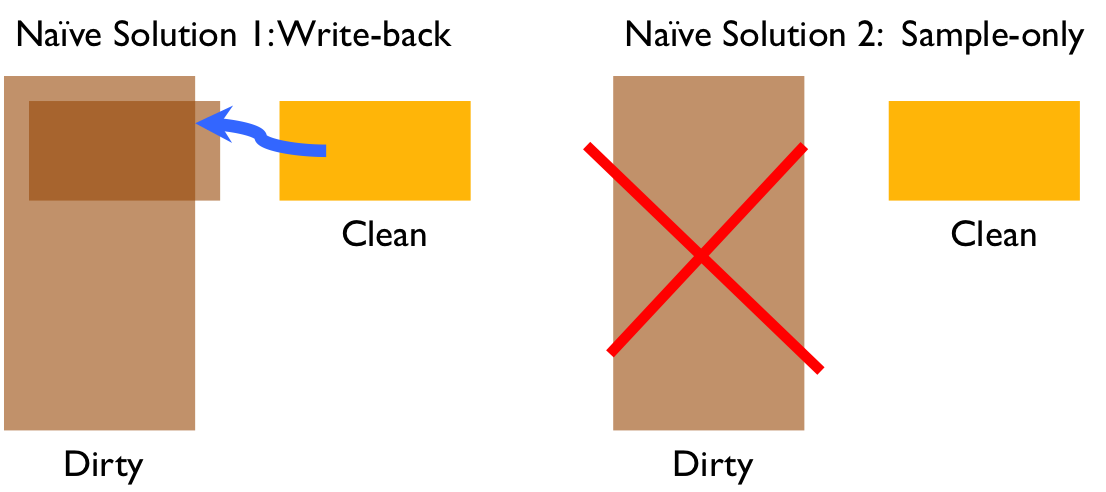
\includegraphics[width=\columnwidth]{figs/update-arch.png}
 \caption{(a) Systematic corruption (translation) in one variable where the dirty data is in brown, the clean data is in yellow, and their respective best fit lines are in blue. 
 (b) Applying the same model to mixed data results in an inaccurate model.
(c) Likewise, small sample sizes can result in similarly inaccurate models. \label{update-arch1}}
\end{figure}

An alternative is to avoid the dirty data altogether instead of mixing the two populations.
Suppose $k$ records are randomly sampled from the dataset and cleaned.
The model is trained only on the cleaned sample of data.
This is similar to SampleClean \cite{wang1999sample}, which was proposed to approximate the results of aggregate queries by applying them to a clean sample of data.
However, high-dimensional models are highly sensitive to sample size.
Figure \ref{update-arch1}c illustrates that, even in two dimensions, models trained from small samples can be as incorrect as the mixing solution described before.

In this work, we propose a new methodology to avoid Simpson's Paradox and the strong dependence on sample size.
Instead of mixing dirty and clean data, \sys uses a model trained on the dirty data as an initialization, and then iteratively updates this model using samples of clean data.
The intuition is that this algorithm smoothly transitions the model from one population (the dirty data) to another (the clean data), leading to provable guarantees about intermediate results.

%\sys avoids both pitfalls, Simpson's paradox and sample size dependence.

\iffalse
\sys avoids both pitfalls, Simpson's paradox and sample size dependence.
In Section \ref{model-update}, we show how we do this with iterative gradient steps (i.e., incrementally moving the line based on the clean data).
This takes advantage of the dirty data as well as the clean data, but still have provable properties about the intermediate results.
The intuition is that it smoothly and iteratively transitions the model from one population (the dirty data) to another (the clean data).
In Figure \ref{sys-arch2}, we illustrate our ideal tradeoff space of sampling and data cleaning.
At two extremes we have no cleaning (just using the dirty data) and full cleaning.
%\sys is optimized for convergence for smaller sample sizes than a uniform sampling approach.

\begin{figure}[t]
\centering
 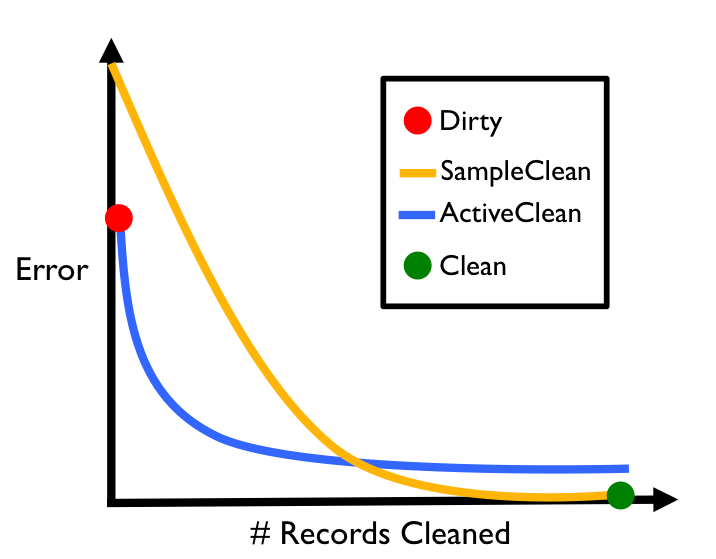
\includegraphics[width=0.5\columnwidth]{figs/arch2.png}
 \caption{\sys is designed to converge to an accurate model with fewer cleaned records than a uniform sampling approach (SampleClean). \label{sys-arch2}}\vspace{-1em}
\end{figure}


We design \sys to make greater progress at these small sample sizes using the dirty model as an initialization.
Doing so is not trivial since it requires analysis of both the Machine Learning model and the data cleaning operations.
Data may look unimportant to a dirty model but when cleaned are very important.
Also, data cleaning and model training can happen at very different time scales, we have to carefully budget our effort to ensure that any optimizations actually address rate-determining steps in the workflow.
Finally, in this line of work, the tradeoff space is enormous, and we have to carefully pick a design point and tailor our optimizations to this preferred regime.
\fi

\subsection{Preliminaries: Convex Data Analytics}
To design an algorithm that avoids Simpson's paradox, this work focuses on an initial class of well analyzed predictive analytics problems; ones that can be expressed as the minimization of convex loss functions.
Convex loss minimization problems are amenable a variety of incremental optimization methodologies with provable guarantees (see Friedman, Hastie, and Tibshirani \cite{friedman2001elements} for an introduction).
Examples includes all generalized linear models (including linear and logistic regression), all variants of support vector machines, and in fact, means and medians are also special cases. 

Formally, for labeled training examples $\{(x_{i},y_{i})\}_{i=1}^{N}$, the problem is to find a vector of \emph{model parameters} $\theta$ by minimizing a loss function $\phi$ over all training examples:
\[
 \theta^{*}=\arg\min_{\theta}\sum_{i=1}^{N}\phi(x_{i},y_{i},\theta)
\]
Where $\phi$ is a convex function in $\theta$.
For example, in a linear regression $\phi$ is:
\[
\phi(x_{i},y_{i},\theta) = \|\theta^Tx_{i} - y_i \|_2^2
\]
Typically, a \emph{regularization} term $r(\theta)$ is added to this problem.
$r(\theta)$ penalizes high or low values of feature weights in $\theta$ to avoid overfitting to noise in the training examples.
\[
 \theta^{*}=\arg\min_{\theta}\sum_{i=1}^{N}\phi(x_{i},y_{i},\theta) + r(\theta)
\]
In this work, without loss of generality, we will include the regularization as part of the loss function i.e., $\phi(x_{i},y_{i},\theta)$ includes $r(\theta)$.

\begin{definition}[Convex Data Analytics]
A convex data analytics problem is specified by a set of features $X$, corresponding set of labels $Y$, and a parametrized loss function $\phi$ that is convex in its parameter $\theta$.
The result is a \textbf{model} $\theta$ that minimizes the sum of losses over all features and labels.
\end{definition}

\subsubsection{Types of Error}
There are two standard metrics to quantify inaccuracy in a model:

\vspace{0.25em}

\noindent\textbf{Model Error. } Let $\theta$ be the model trained on the dirty data, and let $\theta^*$ be the model trained on the same data if all of the records were cleaned. Then the model error is defined as $\|\theta - \theta^*\|$.

\vspace{0.25em}

\noindent\textbf{Testing Error. } Let $\theta$ be the model trained on the dirty data, and let $\theta^*$ be the model trained on the same data if all of the records were cleaned. Let $T(\theta)$ be the out-of-sample testing error when the dirty model is applied to the clean data, and $T(\theta^*)$ be the test error when the clean model is applied to the clean data. The testing error is defined as $T(\theta) - T(\theta^*)$

%\vspace{0.5em}

%\noindent The above \emph{errors} are caused by two underlying problems:

%\vspace{0.25em}

%\noindent\textbf{Data Error. } is error introduced by training a model on systematically corrupted data.

\vspace{0.25em}

\noindent\textbf{Sampling Error. } Error introduced by sampling i.e., the difference between a model trained on $p\%$ of the data and $100\%$ of the data.

\vspace{0.25em}

When we use the term \emph{error}, we are referring to model error.
We will be explicit with other terms when describing data errors (e.g. ``data corruption").

\subsection{\sys Problem}
The core problem addressed by \sys is incremental model update while progressively cleaning data.

\begin{problem}[ActiveClean Problem]\label{activeclean}\sloppy
Let $R$ be a dirty relation, $F(r) \mapsto (x,y)$ be a featurization that maps
a record $r \in R$ to a feature vector $x$ and label $y$, $\phi$ be a convex regularized loss,
and $C(r) \mapsto r_{clean}$ be a cleaning technique that maps a record to its cleaned value. 
Given these inputs, the \sys problem is to return an estimate $\hat{\theta}$ of the clean model for any limit $k$ on the number of times the data cleaning $C(\cdot)$ can be applied.
This estimate should be bounded by a monotonically decreasing function in $k$ (i.e., more cleaning results is expected to improve the model).
\end{problem}

Addressing this problem requires analysis of the loss function $\phi$ and how $\phi$ is affected by dirty data.
The solution is to integrate data cleaning and model training, where $\phi$ is simultaneously minimized while the data is cleaned.
The tight feedback loop between model training and data cleaning poses several new algorithmic challenges and systems challenges.
Algorithmically,  we have to re-weight data to avoid biases and the population mixtures described previously.
There are also numerous new opportunities for optimizations such as prioritizing data and avoiding data that are expected to be clean.

From a systems perspective, data cleaning and model training happen at very different time scales.
When humans are involved, per record latencies for data cleaning are orders of magnitude larger than the CPU time needed for model training.
We can compare recent results in data cleaning to a model training framework like CoCoA implemented on Spark \cite{jaggi2014communication}.
Per record, BigDansing, a highly optimized automated Spark-based data cleaning system is 15.5x slower than CoCoA\footnote{For CoCoA to reach a precision of 1e-3}.
Crowd based techniques like CrowdFill \cite{park2014crowdfill} and CrowdER \cite{wang2012crowder} are over 100,000x slower per record. 
Consequently, all of the optimizations in \sys are designed to address data cleaning latency (i.e., more progress with fewer cleaned records) rather than optimizing for numerical computation (i.e., process fewer records).

\iffalse
Here is an example application of \sys with our running example:
\begin{example}
The analyst first trains her SVM model on the dirty data ignoring the effects of the errors returning a model $\theta^{(d)}$.
She decides that she has a budget of cleaning $100$ records, and decides to clean the 100 records in batches of 10 (set based on how fast she can clean the data, and how often she wants to see an updated result).
She initializes \sys with $\theta^{(d)}$.
\sys samples an initial batch of 10 records.
She manually cleans those records by merging similar drug names, making corporation names consistent, and fixing incorrect labels.
After each batch, the model is updated with the most recent cleaning results $\theta^{(t)}$.
The model improves after each iteration.
After $t=10$ of cleaning, the analyst has an accurate model trained with 100 cleaned records but still utilizes the entire dirty data.
\end{example}



\subsection{Two perspectives on error}
When faced with such errors there are two contrasting perspectives from the Machine Learning and the Database communities.

\vspace{0.5em}

\noindent\textbf{Existing Database Literature. } 
Traditionally, cleaning is agnostic to the queries and analysis that happens downstream. 
This perspective breaks down when cleaning is so expensive that we can only clean a small number of records.
Ideally, we should clean the records that are most valuable to the downstream analysis.

\vspace{0.5em}

\noindent\textbf{Existing  Machine Learning Literature. } The Machine Learning community has focused on
designing models that are robust to outliers (i.e., values far away from the typical value)
For example, in the case of linear regression, we can change the $L_2$ norm to an $L_1$ norm to mitigate the effect of outliers:
\[
\phi(x_{i}^T\theta,y_{i}) = \|\theta^Tx_{i} - y_i \|_1
\]
The quadratic L2 loss implies that examples that deviate far from the typical example are quadratically penalized as opposed to linearly penalized with the L1 loss.
There is a natural tradeoff between robustness and efficiency.
The more robust a technique is, the less efficient it will be (i.e., estimate variance for a fixed number of training examples).
Robust techniques are best suited for random errors that look significantly different the rest of the examples.
When errors are systematic, the Machine Learning answer has been to design features in such a way that they are robust to some systematic bias.
For example, in image processing, scale-invariant feature transforms (SIFT) are widely applied that allow for image models invariant to pose or scaling issues.

\vspace{0.5em}

\noindent\textbf{The \sys Contribution. } We try to bring two perspectives together in this work to address the problem of expensive to clean systematic errors, namely the Database idea of data cleaning and the Machine Learning formalization of empirical risk minimization.
Some errors require expensive cleaning procedures, increasingly using the crowd, and we joint have a time budget on cleaning and analysis.
\sys prioritizes cleaning with respect to an estimated impact on the clean model.



\subsection{SampleClean Project}

Traditionally, data cleaning has explored expensive, up-front cleaning of entire datasets for increased query accuracy.
We proposed the SampleClean problem, in which an analyst cleans a small sample of data, and then estimates the result to an aggregate query e.g., \sumfunc, \countfunc, or \avgfunc.
The main insight from the SampleClean project is that highly accurate answers for aggregate queries does not require cleaning the full dataset.
Generalizing this insight, there is a deep relationship between the application (i.e., the query) and how an analyst should budget their effort in data cleaning.
In fact, \avgfunc and \sumfunc queries are a special case of the convex loss minimization discussed in the previous section:
\[
\phi = (x_{i} - \theta)^2
\]

We then extended the SampleClean work to study cleaning Materialized Views \cite{technicalReport}.
Suppose base data is updated with insertions, deletions, or updates, we explored how we could efficiently propagate
changes to a sample of the view instead of the full view.
Subsequent queries on the view could be answered approximate.

The SampleClean problem inspired an eponymous system that implements sampling, data cleaning, and approximate query processing on the Apache Spark stack \cite{sampleclean}.
Also included in the Apache Spark stack are Machine Learning libraries including MLlib \cite{mllib} and GraphX \cite{graphx}.
The in-memory architecture of the Apache Spark stack allows for increasingly interactive analysis \cite{AgarwalMPMMS13, armbrust2015spark}.
Analysts can prototype data processing workflows on samples to evaluate performance before running expensive batch processing jobs on entire datasets.
With data cleaning and machine learning libraries in the same software ecosystem, we see a new opportunity for joint optimization for interactive model building.



\subsection{Stochastic Gradient Descent}
Sampling is a natural part of any Machine Learning workflow, as stochastic optimization is widely used to fit model parameters.
The problems described in the previous subsections are often trained using a technique called Stochastic Gradient Descent (SGD) or one of its variants.
The basic idea of SGD is to draw a data point at random, calculate the gradient at that point, and then update a current best estimate with that gradient.
\[
\theta^{(t+1)}\leftarrow\theta^{(t)}-\gamma\nabla\phi(x_{i}^T\theta,y_{i})
\]
 SGD can also be applied in a ``mini-batch" mode, where we draw a subset of data $S^{(t)}$ at random and update with the average gradient.
 \[
 \theta^{(t+1)}\leftarrow\theta^{(t)}-\frac{\gamma}{\|S^{(t)}\|}\sum_{i\in S^{(t)}}\nabla\phi(x_{i}^T\theta,y_{i})
 \]

We can use this workflow for designing an anytime data cleaning methodology.
As data is sampled, we can clean the samples.
The analyst then can stop at anytime and use the best model at that instant.
SGD and its variants are well-studied and there are lower-bounds on the convergence rates using these techniques. 
Recently, a number of works have explored non-uniform sampling distributions for stochastic optimization \cite{zhao2014stochastic, qu2014randomized}.
The main insight is that non-uniform distributions may on average estimate the gradient accurately.
In this work, we explore how to design such a non-uniform distribution for iterative data cleaning.

\fi


 